\documentclass[11pt]{article}

\usepackage[margin=1in]{geometry}
\usepackage{amsmath, amssymb, amsthm}
\usepackage{graphicx}
\usepackage{enumitem}
\usepackage{listings} % For including Python code
\usepackage{xcolor}
\usepackage{cite}
\usepackage{url}

% --- Code Listing Settings ---
\definecolor{codegreen}{rgb}{0,0.6,0}
\definecolor{codegray}{rgb}{0.5,0.5,0.5}
\definecolor{codepurple}{rgb}{0.58,0,0.82}
\definecolor{backcolour}{rgb}{0.95,0.95,0.92}

\lstdefinestyle{python}{
    backgroundcolor=\color{backcolour},   
    commentstyle=\color{codegreen},
    keywordstyle=\color{magenta},
    numberstyle=\tiny\color{codegray},
    stringstyle=\color{codepurple},
    basicstyle=\ttfamily\footnotesize,
    breakatwhitespace=false,         
    breaklines=true,                 
    captionpos=b,                    
    keepspaces=true,                 
    numbers=left,                    
    numbersep=5pt,                  
    showspaces=false,                
    showstringspaces=false,
    showtabs=false,                  
    tabsize=2
}
\lstset{style=python}

% --- JSON Language Definition ---
% We define how to parse JSON, but let it inherit your 'mystyle' formatting!
\colorlet{punct}{red!60!black}
\definecolor{delim}{RGB}{20,105,176}
\colorlet{numb}{magenta!60!black}

\lstdefinelanguage{json}{
    showstringspaces=false,
    breaklines=true,
    string=[s]{"}{"},
    stringstyle=\color{codepurple}, % Reuses your Python string color!
    comment=[l]{:},
    commentstyle=\color{delim}, % Colors the colons
    literate=
     *{0}{{{\color{numb}0}}}{1}
      {1}{{{\color{numb}1}}}{1}
      {2}{{{\color{numb}2}}}{1}
      {3}{{{\color{numb}3}}}{1}
      {4}{{{\color{numb}4}}}{1}
      {5}{{{\color{numb}5}}}{1}
      {6}{{{\color{numb}6}}}{1}
      {7}{{{\color{numb}7}}}{1}
      {8}{{{\color{numb}8}}}{1}
      {9}{{{\color{numb}9}}}{1}
      {\{}{{{\color{delim}{\{}}}}{1}
      {\}}{{{\color{delim}{\}}}}}{1}
      {[}{{{\color{delim}{[}}}}{1}
      {]}{{{\color{delim}{]}}}}{1}
}

\newcommand{\course}{16:332:509 Convex Optimization}
\newcommand{\assignment}{Tube-Based Model Predictive Control with Stochastic Optimization via SARAH-M}
\newcommand{\name}{Jeff Barner \& Thomas Trieu}
\newcommand{\datefixed}{\today} 
\newcommand{\realspace}{\mathbb{R}}
\newcommand{\intspace}{\mathbb{Z}}
\newcommand{\norm}[1]{\left|\left|#1\right|\right|}
\newcommand{\mtx}[1]{\mathbf{#1}}
\newcommand{\abs}[1]{\left|#1\right|}
\newcommand{\psd}[1]{\mathbb{S}^{#1}_{+}}
\newcommand{\tenpow}[1]{\times 10^{#1}}

\title{\textbf{\course} \\ \assignment}
\author{\name}
\date{\datefixed}

\begin{document}

\maketitle
\section*{Abstract}

\section{Introduction}
Control systems are increasingly moving towards complex and uncertain environments.
Model Predictive Control (MPC) is the standard for constrained systems, but its standard deterministic form lacks a formal mechanism to handle perturbations.
Tube-Based Stochastic MPC (SMPC) represents a sophisticated evolution, providing a framework for maintaining stability within a defined "tube" of trajectories.

\subsection{Tube-Based MPC}
In tube-based MPC, the system state is decomposed into two distinct components: the nominal system, which is the controlled, deterministic model that ignores noise,
and the error system, which measures the deviation between the plant and the nominal model, caused by stochastic disturbances (perturbations).
By centering an invariant set around the nominal trajectory, the controller ensures that as long as the nominal state is controlled effectively, the true state of the system is guaranteed to remain within the tube boundaries with a certain probability.

\subsection{Robust vs. Stochastic Tubes}
Traditional Robust Tube MPC assumes worst-case bounded disturbances, which often results in overly conservative control actions.
Stochastic Tube MPC relaxes this in three ways:
first, by characterizing the probability distribution of the disturbances;
second, by shrinking the constraints based on a risk budget rather than the maximum possible perturbation;
and thirdly, by allowing the system to operate closer to its physical limits, improving the performance without sacrificing the safety margin.

\subsection{Objective} %@Thomas fill this part out
This paper seeks to determine the feasibility of Tube-Based SMPC in practical applications.
First, the authors will outline the application of a Robust Tube MPC for a simple spring-damper system.
% @Thomas I have no idea what you actually did
Next, the authors will implement a tube based SMPC.
Finally, the authors will compare the performance profile of the tube-based SMPC to a Robust Tube MPC.

\section{Technical Background}
\subsection{State-Space Equation}
\begin{figure}
    \centering
    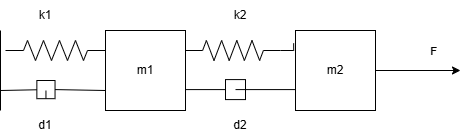
\includegraphics[width=\textwidth]{spring_damper_system.png}
    \label{spring-damper-system}
    \caption{Spring-damper system model.}
\end{figure}

Following the work of Haber\cite{haber2023mpc1}, the physical model of a two-spring, two-damper system is given by Fig.~\ref{spring-damper-system}.
Applying Newton's second law to each mass yields the equations of motion:
$$m_1 \ddot{x}_1 = -(k_1+k_2)x_1 - (d_1+d_2)\dot{x}_1 + k_2 x_2 + d_2 \dot{x}_2$$
$$m_2 \ddot{x}_2 = k_2 x_1 + d_2 \dot{x}_1 - k_2 x_2 - d_2 \dot{x}_2 + F$$

Choose state vector $\mathbf{x} = [x_1, \dot{x}_1, x_2, \dot{x}_2]^\top$, control input $u = F$, and output $y = x_1$.
Then the state-space equation for this system is given by:
$$\dot{\mathbf{x}} = A_c \mathbf{x} + B_c u, \qquad y = C \mathbf{x}$$
here the matrices $A_c$, $B_c$, and $C$ are populated directly from the physical parameters.

The system is then discretized using the forward Euler approximation:
$$A = (I - T_s A_c)^{-1}, \qquad B = A \cdot T_s B_c$$

\subsection{Model Predictive Control}
Model predictive control is an optimization-based control strategy that explicitly uses a dynamic model to predict future plant behavior over a finite prediction horizon $N_p$.
MPC chooses control inputs that minimize a cost function subject to constraints.
At each sampling instant $k$, MPC solves the Optimal Control Problem:

$$\min_{\{u_0, \ldots, u_{N_c-1}\}} \sum_{i=0}^{N_p - 1} \left\| y_{k+i|k} - r_{k+i} \right\|^2_{W_4} + \left\| \Delta u \right\|^2_{W_3}$$
where $y_{k+i|k}$ is the predicted output $i$ steps ahead, $r_{k+i}$ is the reference trajectory, $W_4$ penalizes tracking error over the prediction horizon $N_p$, $W_3$ penalizes control input increments over the control horizon $N_c$, and $\Delta u$ denotes differences between successive control actions.

\section{Main Method}

\section{Numerical Results}

\section{Conclusion}
SMPC can be a viable alternative to Robust MPC 

Repository can be found at: https://github.com/nalddox/convex-optimization-project/

\bibliographystyle{IEEEtran}
\bibliography{references}

\end{document}